% 2025年北京高考数学第17题解析图1：四棱锥P-ABCD
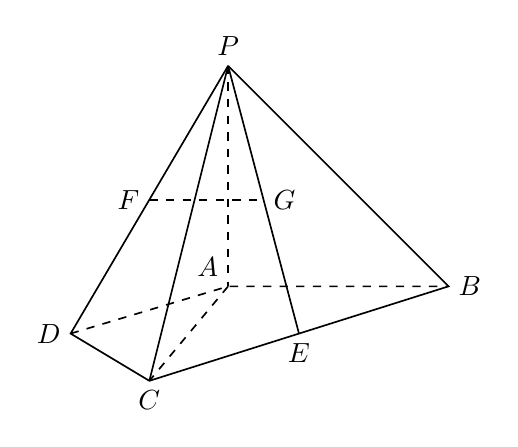
\begin{tikzpicture}[>=stealth,line width=0.6pt,font=\normalsize]
  \coordinate (A) at (1.6,0.6);
  \coordinate (B) at (4.4,0.6);
  \coordinate (C) at (0.6,-0.6);
  \coordinate (D) at (-0.4,0);
  \coordinate (P) at (1.6,3.4);
  \coordinate (E) at (2.5,0);
  \coordinate (F) at (0.6,1.7);
  \coordinate (G) at (2.05,1.7);

  % 实线可见边
  \draw (P) -- (D) -- (C) -- (B) -- (P);
  \draw (P) -- (C);
  \draw (P) -- (E);

  % 虚线不可见底边与截线
  \draw[dashed] (D) -- (A) -- (B);
  \draw[dashed] (P) -- (A);
  \draw[dashed] (A) -- (C);
  \draw[dashed] (F) -- (G);

  % 顶点标注
  \node[above] at (P) {$P$};
  \node[above left] at (A) {$A$};
  \node[right] at (B) {$B$};
  \node[below] at (C) {$C$};
  \node[left] at (D) {$D$};
  \node[below] at (E) {$E$};
  \node[left] at (F) {$F$};
  \node[right] at (G) {$G$};
\end{tikzpicture}
